\chapter{DG 和 STDG的数值实现}
为了数值实现DG以及STDG方法,理论和实现其实并不完全一样。需要说明的是,目前实现DG方法大多以工业软件为主,或者是大型开源的C++库。当然这些都是非常完善的软件,效率也一定非常高。
但是由于接下来想要将其理论和深度学习方法融合,python语言是离不开的。因此有必要用python再实现一些简单的数值算例。而STDG方法目前更是基本没有公开的代码。

下面介绍一些具体实施的细节。
\section{参考单元和真实单元}
在实现DG方法的过程中,可以从理论上看出需要计算在单元上,内切面上的积分,例如三角形,线段等。在这里我们采取在参考单元上的坐标变换,只考虑在参考单元上的积分。

\paragraph*{参考三角单元}
我们将参考三角单元记作$\hat{E}$, 它的三个顶点分别为 $(0,0),(1,0),(0,1)$。 对于任意一个三角单元来说 $E$, 我们有仿射变换 $F_E:\hat{E}\rightarrow E$.
假设E的三个顶点分别为 $(x_i, y_i),i=1,2,3$, 那么我们有
$$
\begin{pmatrix}
    x\\y
\end{pmatrix} = F_E\begin{pmatrix}
    \hat{x}\\ 
    \hat{y}
\end{pmatrix}=B_E\begin{pmatrix}
    \hat{x}\\ 
    \hat{y}
\end{pmatrix}+b_E=\begin{pmatrix}
    x_2-x_1 & x_3-x_1\\
    y_2-y_1 & y_3-y_1
\end{pmatrix}\begin{pmatrix}
    \hat{x}\\ 
    \hat{y}
\end{pmatrix}+\begin{pmatrix}
    x_1\\y_1
\end{pmatrix}
$$ 
简单示意图如下:
\begin{center}
    \begin{tikzpicture}
        \draw (0,0)--(2,0) -- (0,2) --(0,0);
        \node at (4,1.2) {$F_E$};
        \draw[->] (3,1)--(5,1);
        \draw (6,0)--(9,0)--(8,2)--(6,0);
    \end{tikzpicture}
\end{center}

自然的我们有逆变换: 
$$
\begin{pmatrix}
    \hat{x}\\ 
    \hat{y}
\end{pmatrix} = F_E^{-1}\begin{pmatrix}
x\\y
\end{pmatrix}=B_E^{-1}\left(\begin{pmatrix}
    x\\ 
    y
\end{pmatrix}-b_E\right)
$$ 

同时我们可以发现$B_E$的行列式的值在积分计算中有出现。若将$|E|$记作单元E的面积, 那么我们有
$$det(B_E)=2|B_E|$$

因此当我们有定义在参考单元 $\hat{E}$上的函数$\hat{v}$时,有 
$$\hat{v}=v\circ F_E; \qquad v = \hat{v}\circ F_E^{-1}$$

因此$v$ 和 $\hat{v}$的梯度有如下关系:
$$\nabla \hat{v} = B_E^T \nabla v\circ F_E;\qquad \nabla v = B_E^{-T}\nabla \hat{v}\circ F_E^{-1}$$

\section{基函数}
在这里我们设局部基函数为阶数不超过K的多项式。例如
$$\hat{\phi}_i(\hat{x}, \hat{y})=\hat{x}^i\hat{y}^j,i+j=k$$
那么基函数空间项数为 $N_{loc}=\frac{(k+1)(k+2)}{2}$.
\\
具体来说我们有如下几种常用的基函数空间,以2维为例:

分段线性函数:
$$\hat{\phi}_{0}(\hat{x}, \hat{y})=1,  \hat{\phi}_{1}(\hat{x}, \hat{y})=\hat{x}, \hat{\phi}_{2}(\hat{x}, \hat{y})=\hat{y}$$

分段二次函数:
$$\hat{\phi}_{0}(\hat{x}, \hat{y})=1,  \hat{\phi}_{1}(\hat{x}, \hat{y})=\hat{x}, \hat{\phi}_{2}(\hat{x}, \hat{y})=\hat{y},
\hat{\phi}_{3}(\hat{x}, \hat{y})=\hat{x}^{2}, \hat{\phi}_{4}(\hat{x}, \hat{y})=\hat{x} \hat{y}, \hat{\phi}_{5}(\hat{x}, \hat{y})=\hat{y}^{2} .
$$

\section{数值积分}
由于映射$F_E : \hat{E} \rightarrow E $为仿射变换, 并且我们有
$$\int_{E} v=\int_{\hat{E}} v \circ F_{E} \operatorname{det}\left(\boldsymbol{B}_{E}\right)=2|E| \int_{\hat{E}} \hat{v} .$$

那么积分可以由如下方式逼近:

$$\int_{E} v \approx 2|E| \sum_{j=1}^{Q_{\mathrm{D}}} w_{j} \hat{v}\left(s_{x, j}, s_{y, j}\right) .$$


若积分设计向量函数和梯度,则有

$$\begin{aligned}
\int_{E} \nabla u \cdot \boldsymbol{v} & =2|E| \int_{\hat{E}}\left(\boldsymbol{B}_{E}^{T}\right)^{-1} \nabla \hat{u} \cdot \hat{\boldsymbol{v}} \\
& \approx 2|E| \sum_{j=1}^{Q_{\mathrm{D}}} w_{j}\left(\boldsymbol{B}_{E}^{T}\right)^{-1} \nabla \hat{u}\left(s_{x, j}, s_{y, j}\right) \cdot \hat{\boldsymbol{v}}\left(s_{x, j}, s_{y, j}\right) .
\end{aligned}$$

类似的,如果积分关于v,w的梯度都有涉及,我们有
$$\int_{E} \nabla u \cdot \nabla v \approx 2|E| \sum_{j=1}^{Q_{\mathrm{D}}} v_{j}\left(\boldsymbol{B}_{E}^{T}\right)^{-1} \nabla \hat{u}\left(s_{x, j}, s_{y, j}\right) \cdot\left(\boldsymbol{B}_{E}^{T}\right)^{-1} \nabla \hat{v}\left(s_{x, j}, s_{y, j}\right) .$$

\section{DG 数值装配方案}
\subsection{一些细节}
对于理论部分所述关于利用DG方法求解Possion方程部分,我们设计了对称系数以及惩罚因子$\epsilon, \sigma_0$,并且有如下结论:
\begin{itemize}
    \item 若  $\epsilon=-1$ , 方法变为对称型内罚伽辽金方法(symmetric interior penalty Galerkin)。这种方法在惩罚因子$\sigma$足够大的时候收敛。
    \item 若  $\epsilon=+1$ , 方法变为非对称型内罚伽辽金方法 (nonsymmetric interior penalty Galerkin).方法对于任意非负惩罚因子$\sigma_{e}^{0}$都收敛。
    \item 若  $\epsilon=0$ , 方法变为缺型内罚伽辽金方法  (incomplete interior penalty Galerkin). 这种方法在惩罚因子$\sigma$足够大的时候收敛。
    \item $J_{1}$是额外的稳定项。 对于这一项中的惩罚因子$\sigma^1$通常设为0。
\end{itemize}

首先我们将 $A_h(u,v)$ 分为两部分: 
$$\left\{\begin{aligned}
    &T_1 =  (a \nabla u, \nabla v)_{\mathscr{T}_{h}}\\
    &T_2 = -\left(\langle\{a\textbf{n}\cdot \nabla u \},[v]\rangle_{\mathcal{E}_{h}^{I D}}-\epsilon\langle\{a \textbf{n}\cdot\nabla v \}, [u]\rangle_{\mathcal{E}_{h}^{I D}}\right)+\sum_{e \in \mathcal{E}_{h}^{I D}}\frac{\sigma_{e}^{0}}{|e|^{\beta_{0}}} \int_{e}\left[u\right][v]\\
\end{aligned}\right.$$
因此我们有

$$\forall 1 \leq i, j \leq N_{\mathrm{loc}}, \quad\left(T_1\right)_{i, j}=\int_{E}\left( \nabla \phi_{j, E} \cdot \nabla \phi_{i, E}\right)$$

施加坐标仿射变换$F_{E}$, 我们能够将参考单元上的积分算出:

$$\left(T_1\right)_{i, j}=2|E| \int_{\hat{E}}\left(\left(\boldsymbol{B}_{E}^{T}\right)^{-1} \hat{\nabla} \hat{\phi}_{i} \cdot\left(\boldsymbol{B}_{E}^{T}\right)^{-1} \hat{\nabla} \hat{\phi}_{j}\right) .$$

右边项 $ \boldsymbol{b}_{E}$ 对应的可以写为

$$\left(\boldsymbol{b}_{E}\right)_{i}=\int_{E} f \phi_{i, E} = det(B_E)\int_{\hat{E}} f \hat{\phi}_i.$$

现在我们可以计算对一个固定的内切面e上积分所对应的局部矩阵:

$$T_2= -\left(\langle\{a\textbf{n}\cdot \nabla u \},[v]\rangle_{\mathcal{E}_{h}^{I D}}-\epsilon\langle\{a \textbf{n}\cdot\nabla v \}, [u]\rangle_{\mathcal{E}_{h}^{I D}}\right)+\sum_{e \in \mathcal{E}_{h}^{I D}}\frac{\sigma_{e}^{0}}{|e|^{\beta_{0}}} \int_{e}\left[u\right][v] .$$

记 $u$ 和  v  限制在单元  $E_{i}$上的函数为$u_{i}$ 和 $ v_{i}$。写成跳量形式并展开,我们可以得到:

若 e 为输入内部的内切面:
$$T_e=-\int_{e}\left\{ \nabla u \cdot \boldsymbol{n}_{e}\right\}[v]+\epsilon \int_{e}\left\{ \nabla v \cdot \boldsymbol{n}_{e}\right\}\left[u\right]+\frac{\sigma_{e}^{0}}{|e|^{\beta_{0}}} \int_{e}\left[u\right][v] .$$
那么其可以写为
$$T_e=m_{e}^{11}+m_{e}^{22}+m_{e}^{12}+m_{e}^{21}$$ 其中
$$\left\{
\begin{aligned}
    &m_{e}^{11}=-\frac{1}{2} \int_{e}  \nabla u_{h, 1} \cdot \boldsymbol{n}_{e} v_{1}+\frac{\epsilon}{2} \int_{e}  \nabla v_{1} \cdot \boldsymbol{n}_{e} u_{h, 1}+\frac{\sigma_{e}^{0}}{|e|^{\beta_{0}}} \int_{e} u_{h, 1} v_{1}, \\
    &m_{e}^{22}=\frac{1}{2} \int_{e}  \nabla u_{h, 2} \cdot \boldsymbol{n}_{e} v_{2}-\frac{\epsilon}{2} \int_{e}  \nabla v_{2} \cdot \boldsymbol{n}_{e} u_{h, 2}+\frac{\sigma_{e}^{0}}{|e|^{\beta_{0}}} \int_{e} u_{h, 2} v_{2}, \\
    &m_{e}^{12}=-\frac{1}{2} \int_{e}  \nabla u_{h, 2} \cdot \boldsymbol{n}_{e} v_{1}-\frac{\epsilon}{2} \int_{e}  \nabla v_{1} \cdot \boldsymbol{n}_{e} u_{h, 2}-\frac{\sigma_{e}^{0}}{|e|^{\beta_{0}}} \int_{e} u_{h, 2} v_{1}, \\
    &m_{e}^{21}=-\frac{1}{2} \int_{e}  \nabla u_{h, 1} \cdot \boldsymbol{n}_{e} v_{2}+\frac{\epsilon}{2} \int_{e}  \nabla v_{2} \cdot \boldsymbol{n}_{e} u_{h, 1}-\frac{\sigma_{e}^{0}}{|e|^{\beta_{0}}} \int_{e} u_{h, 1} v_{2} .
\end{aligned}\right.$$

这四项都是大小为$N_{loc}\times N_{loc}$的二维局部矩阵, 即可以记为 $M_e^{11},M_e^{22},M_e^{12},M_e^{21}$, 因此我们将基函数分别代入可以得到:
$$\left\{
    \begin{aligned}
        &\left(\boldsymbol{M}_{e}^{11}\right)_{i j}=-\frac{1}{2} \int_{e}  \nabla \phi_{j, E_{e}^{1}} \cdot \boldsymbol{n}_{e} \phi_{i, E_{e}^{1}}+\frac{\epsilon}{2} \int_{e}  \nabla \phi_{i, E_{e}^{1}} \cdot \boldsymbol{n}_{e} \phi_{j, E_{e}^{1}}+\frac{\sigma_{e}^{0}}{|e|^{\beta_{0}}} \int_{e} \phi_{j, E_{e}^{1}} \phi_{i, E_{e}^{1}}\\
        &\left(\boldsymbol{M}_{e}^{22}\right)_{i j}=\frac{1}{2} \int_{e}  \nabla \phi_{j, E_{e}^{2}} \cdot \boldsymbol{n}_{e} \phi_{i, E_{e}^{2}}-\frac{\epsilon}{2} \int_{e}  \nabla \phi_{i, E_{e}^{2}} \cdot \boldsymbol{n}_{e} \phi_{j, E_{e}^{2}}+\frac{\sigma_{e}^{0}}{|e|^{\beta_{0}}} \int_{e} \phi_{j, E_{e}^{2}} \phi_{i, E_{e}^{2}}\\
        &\left(\boldsymbol{M}_{e}^{12}\right)_{i j} =-\frac{1}{2} \int_{e}  \nabla \phi_{j, E_{e}^{2}} \cdot \boldsymbol{n}_{e} \phi_{i, E_{e}^{1}}-\frac{\epsilon}{2} \int_{e}  \nabla \phi_{i, E_{e}^{1}} \cdot \boldsymbol{n}_{e} \phi_{j, E_{e}^{2}}-\frac{\sigma_{e}^{0}}{|e|^{\beta_{0}}} \int_{e} \phi_{j, E_{e}^{2}} \phi_{i, E_{e}^{1}}\\
        &\left(\boldsymbol{M}_{e}^{21}\right)_{i j} =\frac{1}{2} \int_{e}  \nabla \phi_{j, E_{e}^{1}} \cdot \boldsymbol{n}_{e} \phi_{i, E_{e}^{2}}+\frac{\epsilon}{2} \int_{e}  \nabla \phi_{i, E_{e}^{2}} \cdot \boldsymbol{n}_{e} \phi_{j, E_{e}^{1}}-\frac{\sigma_{e}^{0}}{|e|^{\beta_{0}}} \int_{e} \phi_{j, E_{e}^{1}} \phi_{i, E_{e}^{2}} 
    \end{aligned}
\right.$$

若 e 为属于边界上的内切面, 那么我们只有
$$\left(\boldsymbol{M}_{e}^{11}\right)_{i j}=-\int_{e}  \nabla \phi_{j, E_{e}^{1}} \cdot \boldsymbol{n}_{e} \phi_{i, E_{e}^{1}}+\epsilon\int_{e}  \nabla \phi_{i, E_{e}^{1}} \cdot \boldsymbol{n}_{e} \phi_{j, E_{e}^{1}}+\frac{\sigma_{e}^{0}}{|e|^{\beta_{0}}} \int_{e} \phi_{j, E_{e}^{1}} \phi_{i, E_{e}^{1}}$$
并且局部的右端项 $b_e$ 为 
$$(b_e)_i=\epsilon\int_e\left(\nabla \phi_{i,E_{e}^1}\cdot \boldsymbol{n}_{e}+\frac{\sigma_{e}^{0}}{|e|^{\beta_{0}}}\phi_{i, E_{e}^{1}}\right)g_D$$

在这里我们设 $\beta_0=1, \sigma_0 = 10*p^2, \epsilon=-1$

\subsection{数值结果}
编写语言:Python 3.11 
\subsubsection*{1D 问题}
我们假设精确的解析解为$u(x) = (1-x)e^{-x^2}$. 

下面分别是利用DG方法求出的数值解和精确解的图像
\begin{figure}[H]
    \centering  
    \begin{subfigure}{0.5\textwidth}  
        \centering  
        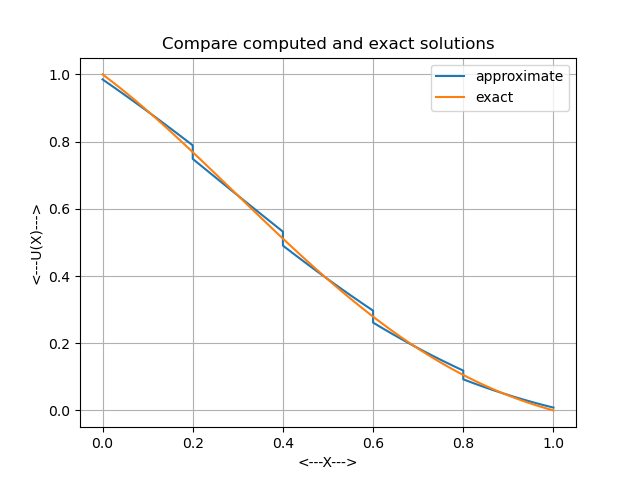
\includegraphics[width=0.9\linewidth]{./pics/final/possion/1d/n5ss-1p1.png}  
        \caption{5 verticles with SIPG $\sigma=1$}  
    \end{subfigure}%  
    \begin{subfigure}{0.5\textwidth}  
        \centering  
        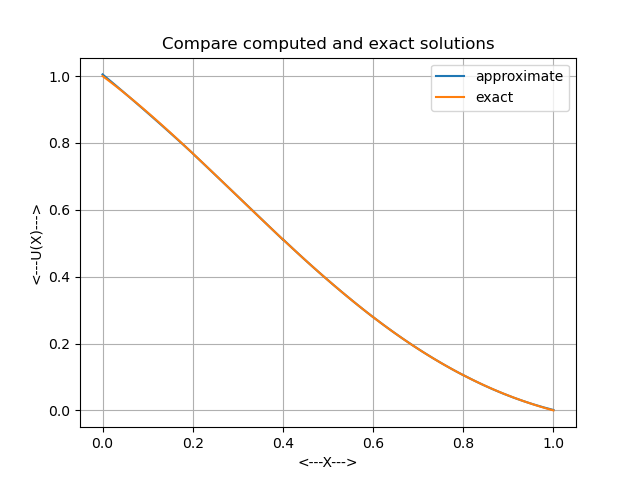
\includegraphics[width=0.9\linewidth]{./pics/final/possion/1d/n5ss-1p5.png}  
        \caption{5 verticles with SIPG $\sigma=5$}
    \end{subfigure}  
    \caption{SIPG}  
\end{figure} 

\begin{figure}[H]
    \centering  
    \begin{subfigure}{0.5\textwidth}  
        \centering  
        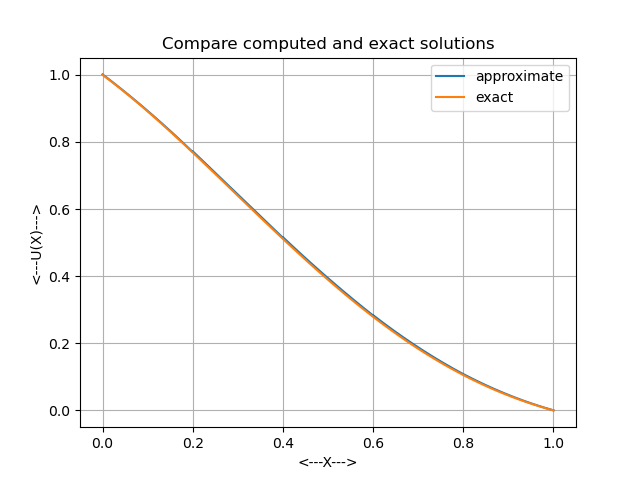
\includegraphics[width=0.9\linewidth]{./pics/final/possion/1d/n5ss1p1.png}  
        \caption{5 verticles with NIPG $\sigma=1$}  
    \end{subfigure}%  
    \begin{subfigure}{0.5\textwidth}  
        \centering  
        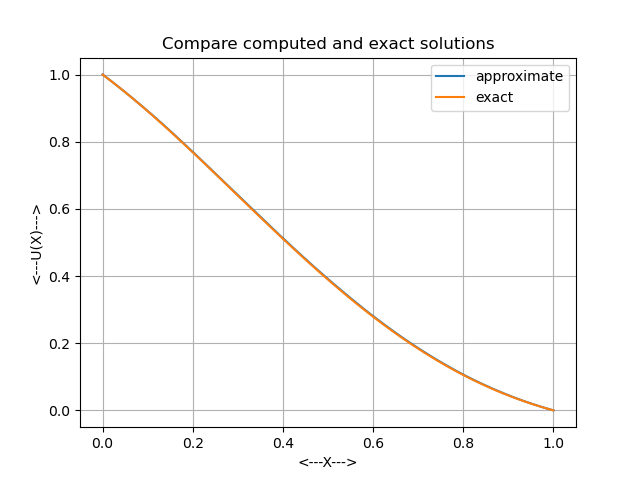
\includegraphics[width=0.9\linewidth]{./pics/final/possion/1d/n5ss1p5.png}  
        \caption{5 verticles with NIPG $\sigma=5$}
    \end{subfigure}  
    \caption{NIPG}  
\end{figure} 

\subsubsection*{2D 问题}
在这里我们使用了python中Triangle 库来生成 2D网格,具体的参数设置见附录。 我们可以通过设置每个单元,三角形,的最大的面积以及生成的最大角度来控制我们想要的三角划分,同时它提供了生成不规则区域的边界方法。

\subsubsection*{----齐次狄利克雷边界----}
下面是有齐次边界条件的Possion方程解的3D以及热力示意图,其中 $f=1$

\begin{figure}[H]
    \centering  
    \begin{subfigure}{0.5\textwidth}  
        \centering  
        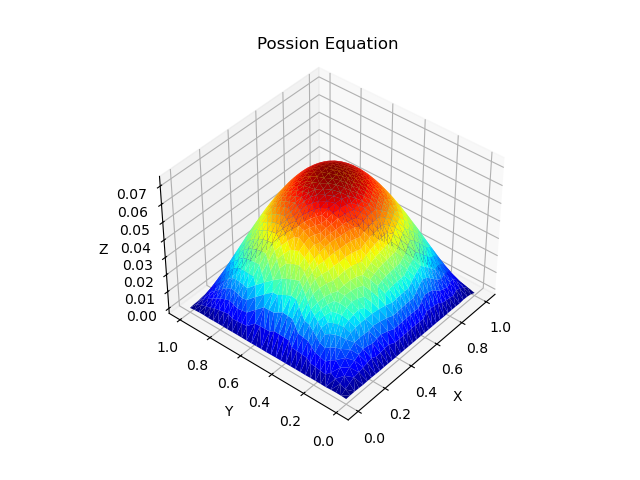
\includegraphics[width=0.9\linewidth]{./pics/final/possion/2d/3Dplot_eps-1.0sig10.0_parapq30a0.01e.png}  
        \caption{SIPG $\sigma=10$}  
    \end{subfigure}%  
    \begin{subfigure}{0.5\textwidth}  
        \centering  
        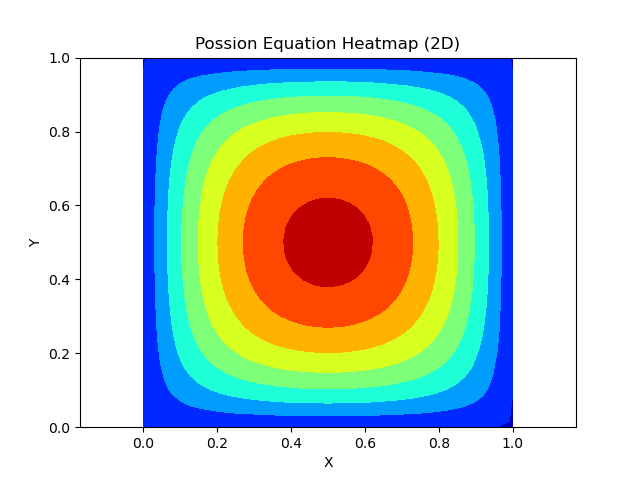
\includegraphics[width=0.9\linewidth]{./pics/final/possion/2d/heatmap_eps-1.0sig10.0_parapq30a0.01e.png}  
        \caption{SIPG $\sigma=10$}
    \end{subfigure}  
    \caption{SIPG}  

    \begin{subfigure}{0.5\textwidth}  
        \centering  
        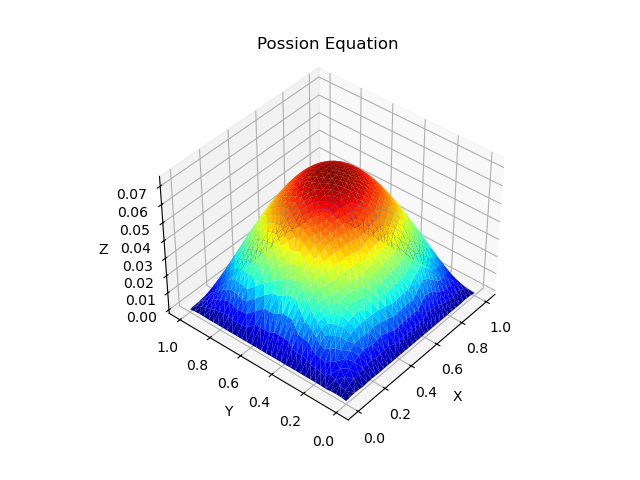
\includegraphics[width=0.9\linewidth]{./pics/final/possion/2d/3Dplot_eps1.0sig10.0_parapq30a0.01e.png}  
        \caption{NIPG $\sigma=10$}  
    \end{subfigure}%  
    \begin{subfigure}{0.5\textwidth}  
        \centering  
        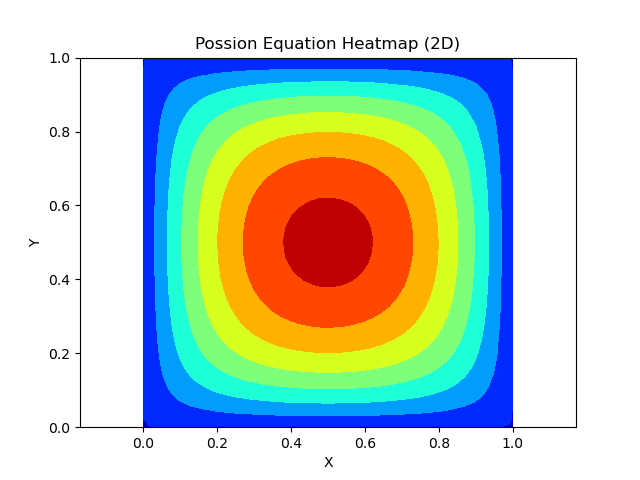
\includegraphics[width=0.9\linewidth]{./pics/final/possion/2d/heatmap_eps1.0sig10.0_parapq30a0.01e.png}  
        \caption{NIPG $\sigma=10$}
    \end{subfigure}  
    \caption{NIPG}  
\end{figure} 

\begin{figure}[H]
    \centering  
    \begin{subfigure}{0.5\textwidth}  
        \centering  
        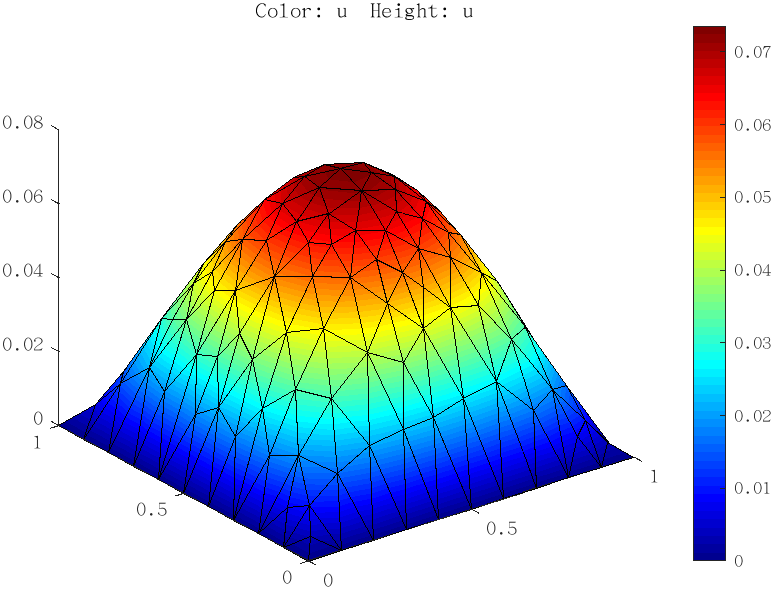
\includegraphics[width=0.9\linewidth]{./pics/final/possion/2d/matlabf13D.png}  
        \caption{3D plot by matlab}  
    \end{subfigure}%  
    \begin{subfigure}{0.5\textwidth}  
        \centering  
        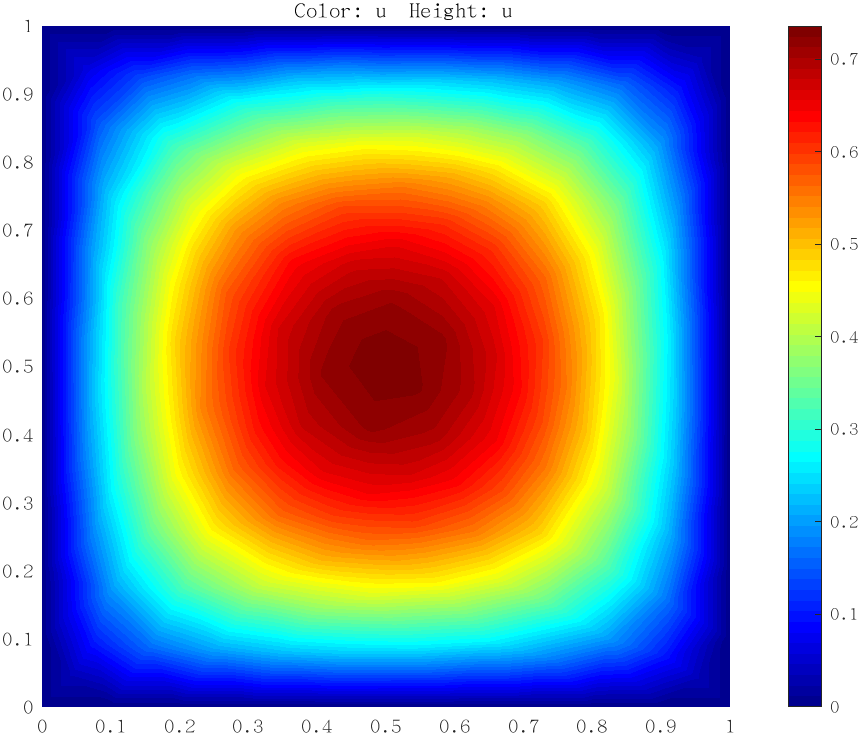
\includegraphics[width=0.9\linewidth]{./pics/final/possion/2d/matlabf1heatmap.png}  
        \caption{heat map by matlab}
    \end{subfigure}  
\end{figure} 

\subsubsection*{----$u(x,y)=e^{-x^2-y^2}$----}
解析解为$u(x,y)=e^{-x^2-y^2}$,主要考察程序在非其次边界条件是否成立。
\begin{figure}[H]
    \centering  
    \begin{subfigure}{0.5\textwidth}  
        \centering  
        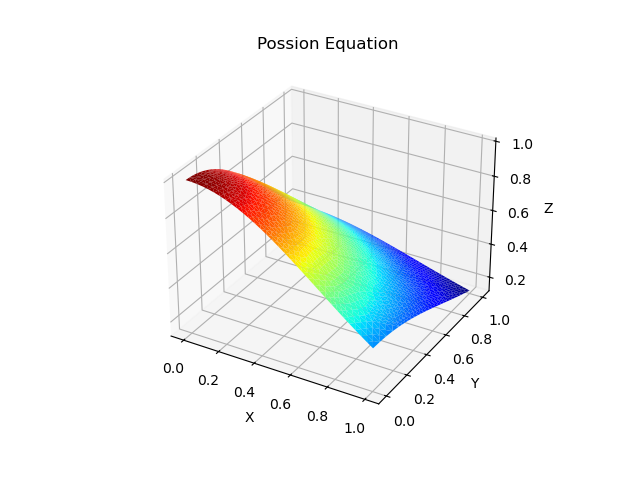
\includegraphics[width=0.9\linewidth]{./pics/final/possion/2d/3Dplot_ex.png}  
        \caption{3Dplot}  
    \end{subfigure}%  
    \begin{subfigure}{0.5\textwidth}  
        \centering  
        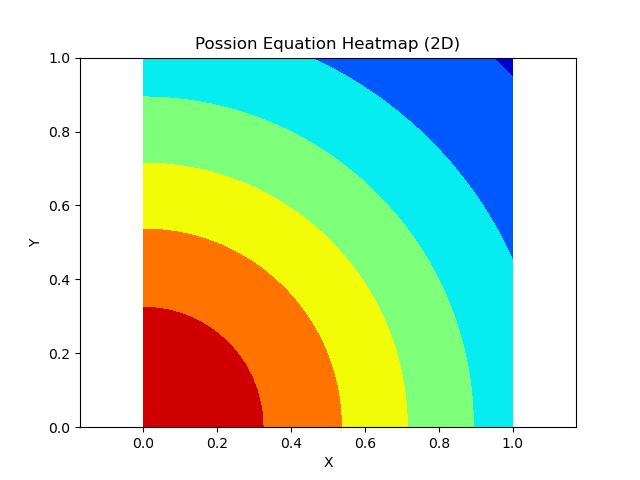
\includegraphics[width=0.9\linewidth]{./pics/final/possion/2d/heatmap_ex.png}  
        \caption{heatmap}
    \end{subfigure}  
    \caption{SIPG}  

    \begin{subfigure}{0.5\textwidth}  
        \centering  
        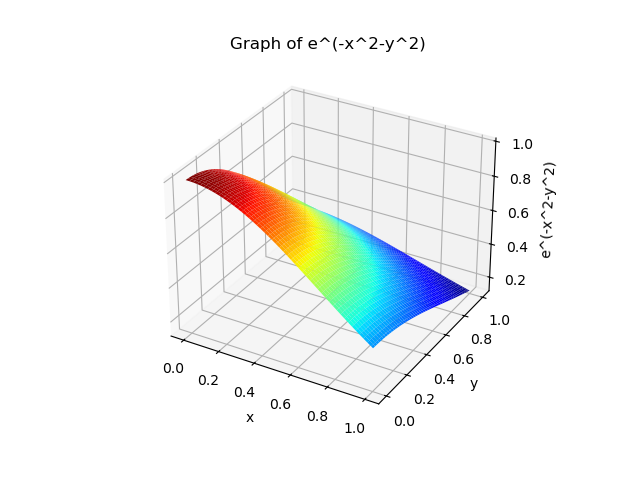
\includegraphics[width=0.9\linewidth]{./pics/final/possion/2d/true3D.png}  
        \caption{exact 3D}  
    \end{subfigure}%  
    \begin{subfigure}{0.5\textwidth}  
        \centering  
        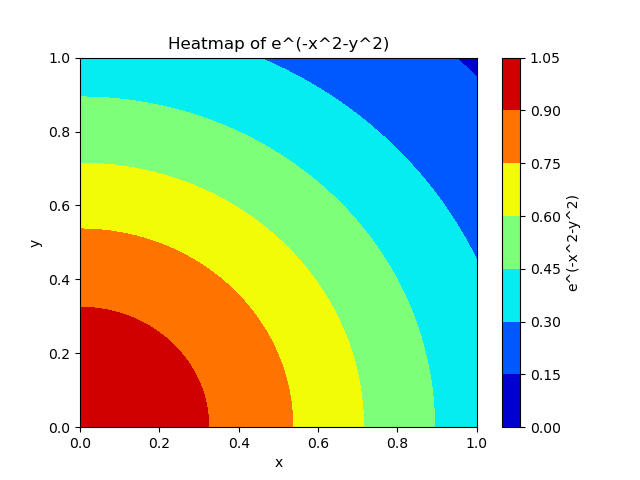
\includegraphics[width=0.9\linewidth]{./pics/final/possion/2d/trueheat.png}  
        \caption{Exact heat}
    \end{subfigure} 
\end{figure} 

\subsubsection*{----不规则边界----}.
$f=10$ with homogeneous dirichlet boundary condition.
\begin{figure}[H]
    \centering  
    \begin{subfigure}{0.5\textwidth}  
        \centering  
        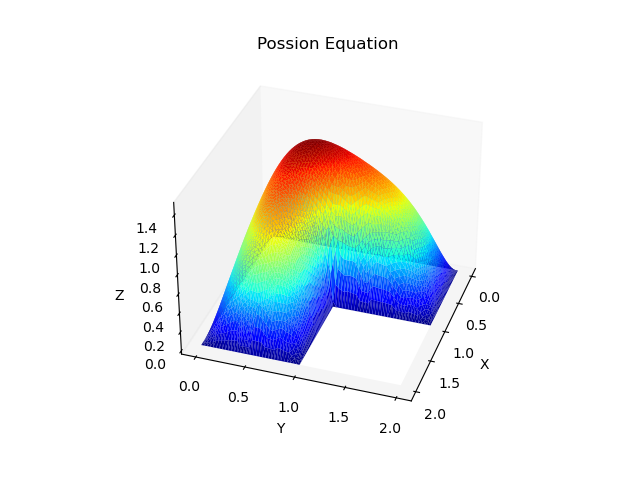
\includegraphics[width=0.9\linewidth]{./pics/final/possion/2d/irregularmine3D.png}  
        \caption{3Dplot}  
    \end{subfigure}%  
    \begin{subfigure}{0.5\textwidth}  
        \centering  
        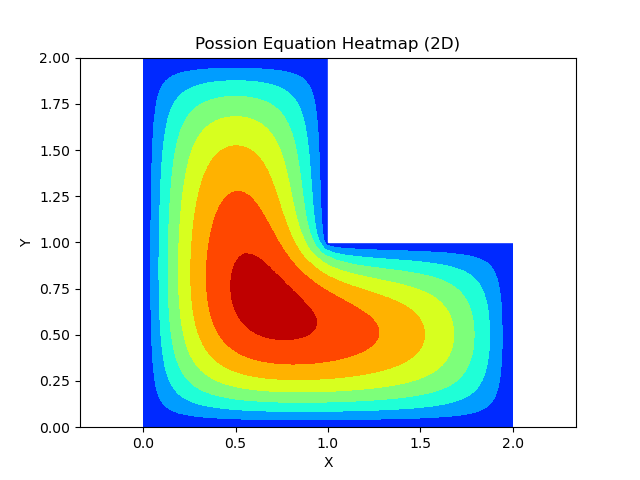
\includegraphics[width=0.9\linewidth]{./pics/final/possion/2d/irregularmineheat.png}  
        \caption{heatmap}
    \end{subfigure}  

    \begin{subfigure}{0.5\textwidth}  
        \centering  
        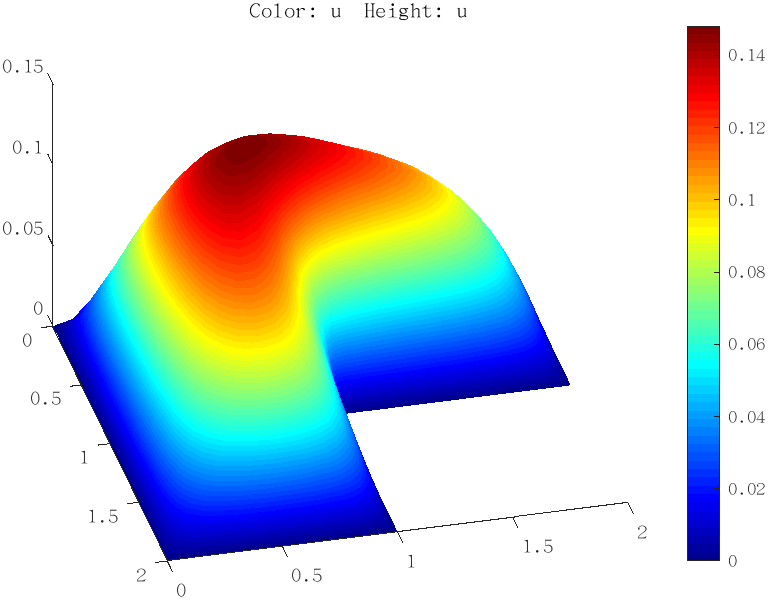
\includegraphics[width=0.9\linewidth]{./pics/final/possion/2d/matlabirregular3D.png}  
        \caption{matlab 3D}  
    \end{subfigure}%  
    \begin{subfigure}{0.5\textwidth}  
        \centering  
        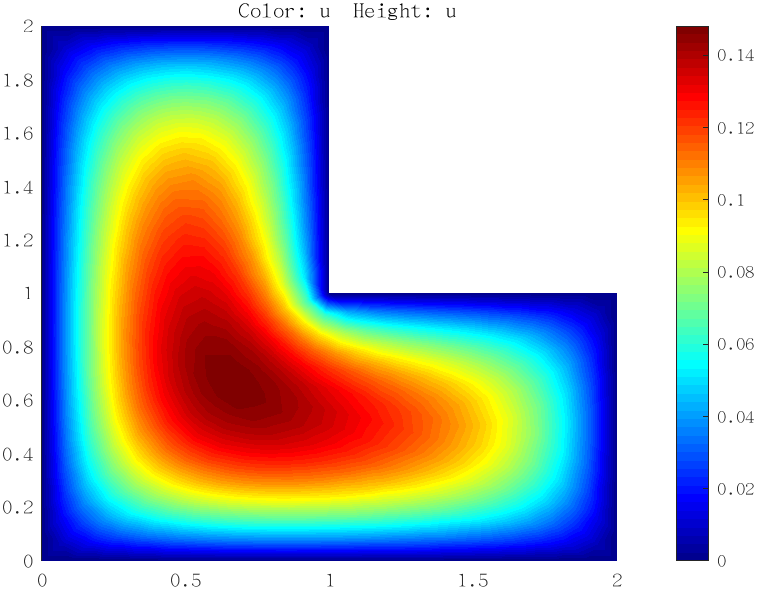
\includegraphics[width=0.9\linewidth]{./pics/final/possion/2d/matlabirregularheat.png}  
        \caption{matlab heat}
    \end{subfigure} 
\end{figure} 

\subsubsection*{----有奇点情况----}.
解析解为$(x^2+(y-\frac{1}{2})^2)^{\frac{1}{4}}$
\begin{figure}[H]
    \centering  
    \begin{subfigure}{0.5\textwidth}  
        \centering  
        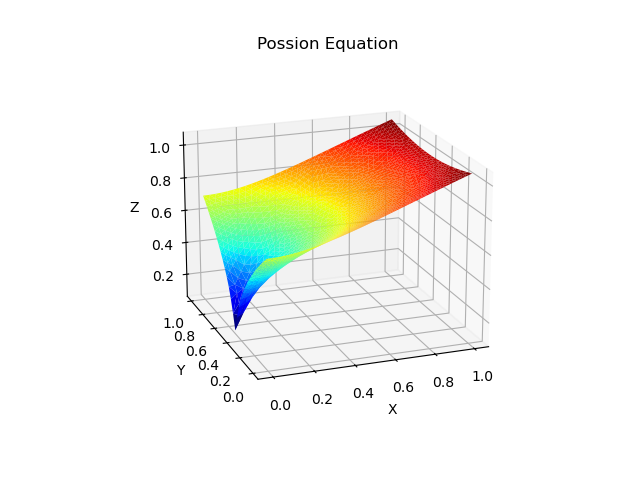
\includegraphics[width=0.9\linewidth]{./pics/final/possion/2d/jumpsol3D.png}  
        \caption{3Dplot}  
    \end{subfigure}%  
    \begin{subfigure}{0.5\textwidth}  
        \centering  
        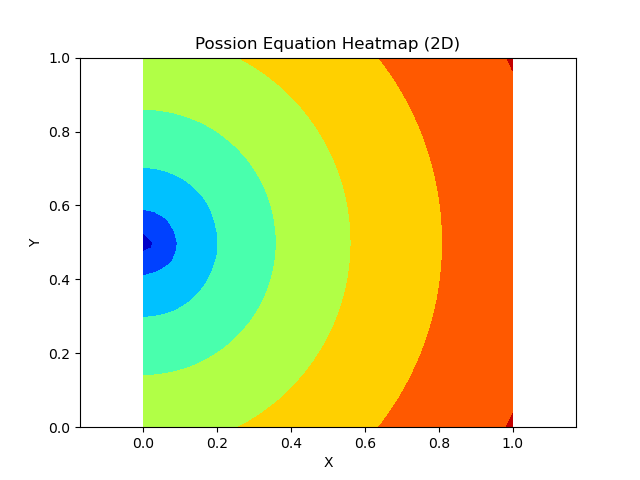
\includegraphics[width=0.9\linewidth]{./pics/final/possion/2d/jumpsolheat.png}  
        \caption{heatmap}
    \end{subfigure}  

    \begin{subfigure}{0.5\textwidth}  
        \centering  
        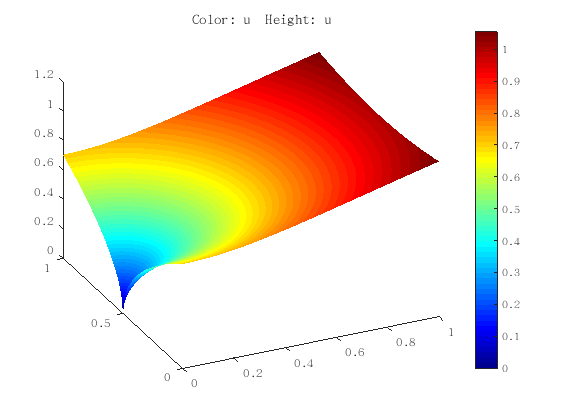
\includegraphics[width=0.9\linewidth]{./pics/final/possion/2d/jumpexact3D.png}  
        \caption{matlab 3D}  
    \end{subfigure}%  
    \begin{subfigure}{0.5\textwidth}  
        \centering  
        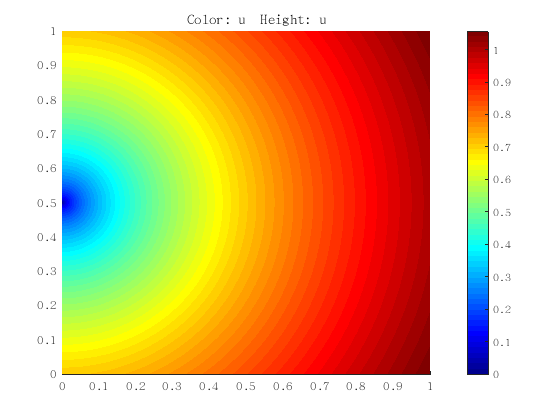
\includegraphics[width=0.9\linewidth]{./pics/final/possion/2d/jumpexactheat.png}  
        \caption{matlab heat}
    \end{subfigure} 
\end{figure} 

\section{时空间断加辽金方法(STDG) 方案}
\subsection{一些细节}
利用时空间断伽辽金方法处理1D问题和上述处理2Dpossion方程有一定的相似之处,但由于原理上有些差异,我们也叙述其求解细节,将其数值实现。 
由 \ref{auv}可见, 我们当然可以以相同的方法得到 $A_E$和$ M_{ij}$. 除此之外, 由(\ref{buv}) 可以得到:

若e 是属于内部的内切面,并且由于迎风量决定我们有当 $n_{E_{e}^1,t}>0$,
$$\left\{
\begin{aligned}
    &(N^{11}_e)_{ij} = \int_e  \phi_{j,E_{e}^1} \phi_{i,E_{e}^1}\cdot n_{E_{e}^1,t}\\
    &(N^{21}_e)_{ij} = -\int_e  \phi_{j,E_{e}^1} \phi_{i,E_{e}^2}\cdot n_{E_{e}^1,t}\\
\end{aligned}
\right.$$

否则 $n_{E_{e}^1,t}$
$$\left\{
\begin{aligned}
    &(N^{12}_e)_{ij} = \int_e  \phi_{j,E_{e}^2} \phi_{i,E_{e}^1}\cdot n_{E_{e}^1,t}\\
    &(N^{22}_e)_{ij} = -\int_e  \phi_{j,E_{e}^2} \phi_{i,E_{e}^2}\cdot n_{E_{e}^1,t}\\
\end{aligned}
\right.$$

若e 是 $\Sigma_T$上的边, 那么可以知道在正方形区域上 $n_{E_{e},t}$ 永远是 1, 因此有:
$$(N_e)_{ij} = \int_e  \phi_{j,E_{e}} \phi_{i,E_{e}}\cdot n_{E_{e},t}$$

在这里值的注意的是我们将涉及$\Sigma_0$上的边上积分移到了右边, 并且将(\ref{buv})的第一项添加到了上面的$A_E$中。
\subsection{数值结果}
\subsubsection{Regular Solution}
解析解为$u(x,t)=cos(\pi t)sin(\pi x)$

\begin{figure}[H]
    \centering  
    \begin{subfigure}{0.5\textwidth}  
        \centering  
        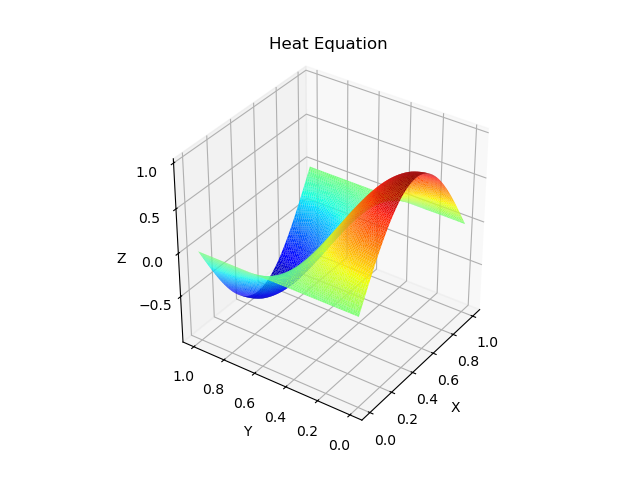
\includegraphics[width=0.9\linewidth]{./pics/final/spacetime/regular/regularmine3D.png}  
        \caption{3Dplot}  
    \end{subfigure}%  
    \begin{subfigure}{0.5\textwidth}  
        \centering  
        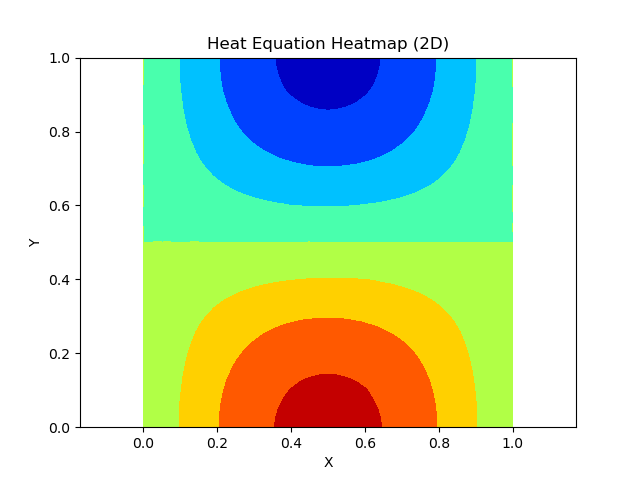
\includegraphics[width=0.9\linewidth]{./pics/final/spacetime/regular/regularmineheat.png}  
        \caption{heatmap}
    \end{subfigure}  

    \begin{subfigure}{0.33\textwidth}  
        \centering  
        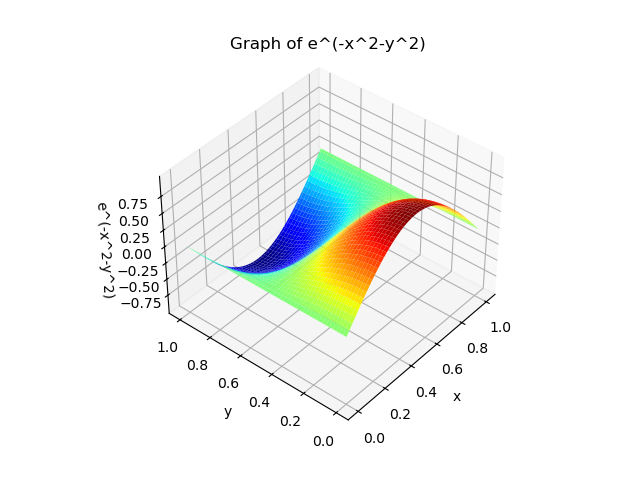
\includegraphics[width=0.9\linewidth]{./pics/final/spacetime/regular/true3D.png}  
        \caption{matlab 3D}  
    \end{subfigure}%  
    \begin{subfigure}{0.33\textwidth}  
        \centering  
        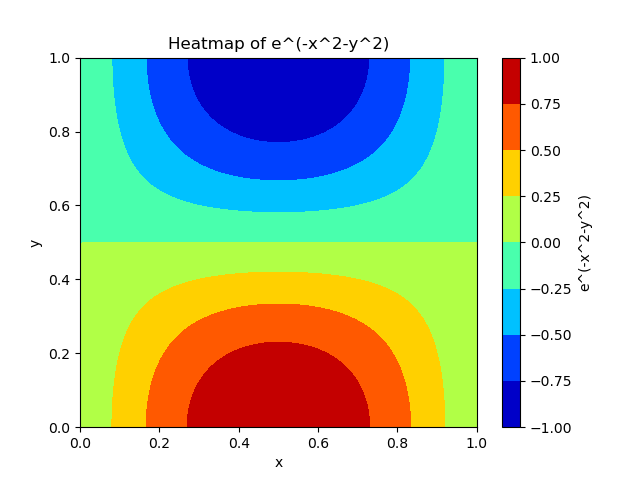
\includegraphics[width=0.9\linewidth]{./pics/final/spacetime/regular/trueheat.png}  
        \caption{matlab heat}
    \end{subfigure} 
    \begin{subfigure}{0.33\textwidth}  
        \centering  
        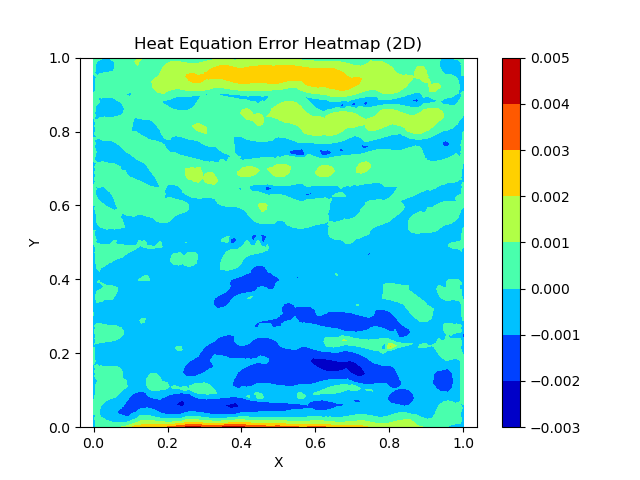
\includegraphics[width=0.9\linewidth]{./pics/final/spacetime/regular/error001.png}  
        \caption{和解析解误差,网格大小0.01}
    \end{subfigure} 
\end{figure} 

$f=1$ 初始条件为$sin(\pi x)$
\begin{figure}[H]
    \centering  
    \begin{subfigure}{0.33\textwidth}  
        \centering  
        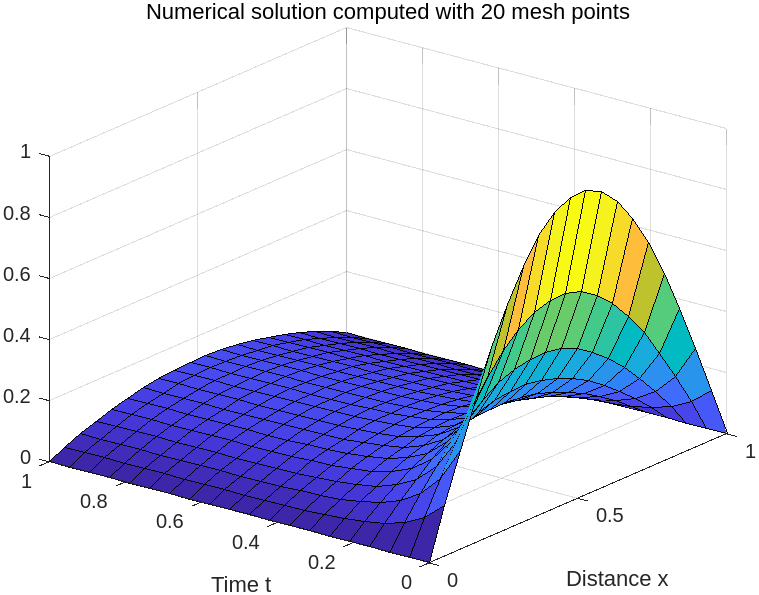
\includegraphics[width=0.9\linewidth]{./pics/final/spacetime/regular/matlabf1.png}  
        \caption{Matlab}
    \end{subfigure}  
    \begin{subfigure}{0.33\textwidth}  
        \centering  
        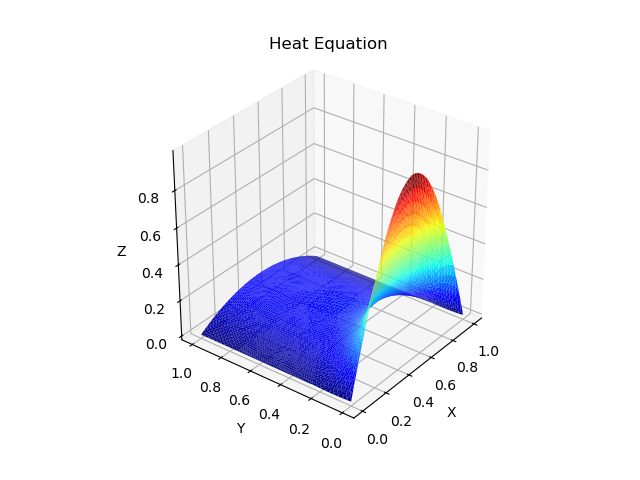
\includegraphics[width=0.9\linewidth]{./pics/final/spacetime/regular/f1.png}  
        \caption{ST Method 3D}  
    \end{subfigure}%  
    \begin{subfigure}{0.33\textwidth}  
        \centering  
        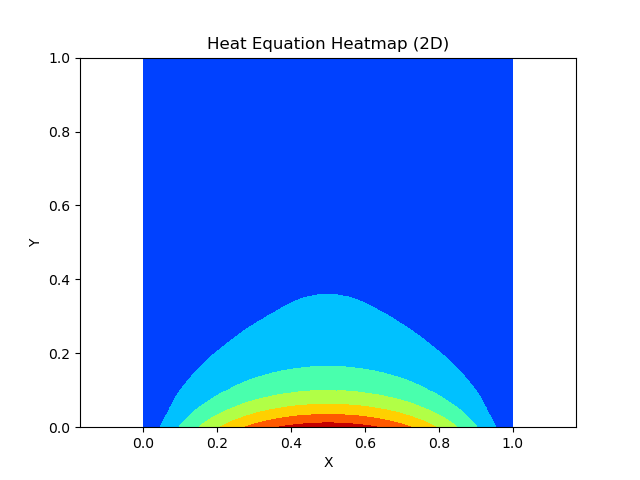
\includegraphics[width=0.9\linewidth]{./pics/final/spacetime/regular/f1heat.png}  
        \caption{ST Method Heat}
    \end{subfigure} 
\end{figure} 

% \subsubsection{irregular solution}
% \paragraph*{$u(x,t)=(x^2+(t-\frac{1}{2})^2)^{\frac{1}{4}}$}. Something went wrong...